\documentclass[12pt,a4paper]{article}

% Paquetes esenciales
\usepackage[utf8]{inputenc}
\usepackage[spanish,es-tabla]{babel}
\usepackage[T1]{fontenc}
\usepackage{geometry}
\usepackage{graphicx}
\usepackage{amsmath}
\usepackage{amssymb}
\usepackage{hyperref}
\usepackage{fancyhdr}
\usepackage{float}
\usepackage{booktabs}
\usepackage{tabularx}
\usepackage{xcolor}
\usepackage{listings}
\usepackage{tikz}
\usetikzlibrary{shapes.geometric, arrows.meta, positioning, calc, backgrounds, fit}

% Configuración de márgenes
\geometry{
    left=2.5cm,
    right=2.5cm,
    top=3cm,
    bottom=3cm
}

% Configuración de colores y enlaces
\definecolor{primary}{RGB}{0, 86, 179}
\definecolor{secondary}{RGB}{108, 117, 125}
\definecolor{codebg}{RGB}{248, 249, 250}
\definecolor{comment}{RGB}{0, 128, 0}
\definecolor{keyword}{RGB}{0, 0, 255}
\definecolor{string}{RGB}{163, 21, 21}

\hypersetup{
    colorlinks=true,
    linkcolor=primary,
    filecolor=magenta,      
    urlcolor=primary,
    pdftitle={Implementación de Autenticación Multifactor (MFA) en Entornos Reales},
    pdfpagemode=FullScreen,
}

% Configuración de listados de código
\lstset{
    backgroundcolor=\color{codebg},   
    commentstyle=\color{comment},
    keywordstyle=\color{keyword},
    numberstyle=\tiny\color{secondary},
    stringstyle=\color{string},
    basicstyle=\ttfamily\footnotesize,
    breakatwhitespace=false,         
    breaklines=true,                 
    captionpos=b,                    
    keepspaces=true,                 
    numbers=left,                    
    numbersep=5pt,                  
    showspaces=false,                
    showstringspaces=false,
    showtabs=false,                  
    tabsize=2,
    frame=single,
    rulecolor=\color{secondary!50}
}

% Estilo de página
\pagestyle{fancy}
\fancyhf{}
\fancyhead[L]{Seguridad Informática}
\fancyhead[R]{Proyecto 2: Autenticación MFA}
\fancyfoot[C]{\thepage}

% Datos del documento
\title{
    \vspace{-2cm}
    \Huge\textbf{Trabajo Final: Implementación de Autenticación Multifactor (MFA) en Entornos Reales}\\
    \vspace{0.5cm}
    \Large\textit{Propuesta 2: Seguridad Informática}
}
\author{}
\date{\today}

\begin{document}

\maketitle
\thispagestyle{empty}

\vspace{2cm}
\begin{abstract}
\noindent El presente documento detalla el diseño, arquitectura, implementación y evaluación de un prototipo funcional de portal web transaccional seguro (``Colombia Store'') que integra un esquema robusto de Autenticación Multifactor (MFA). El sistema implementado mitiga activamente las vulnerabilidades inherentes a los modelos de autenticación tradicional basados exclusivamente en contraseñas estáticas, exigiendo a los usuarios configurar y verificar de manera obligatoria una contraseña de un solo uso basada en tiempo (TOTP) gestionada mediante aplicaciones como Google Authenticator o Authy. Se aborda la problemática del robo de credenciales, se fundamenta teóricamente la elección tecnológica que incluye Node.js, Express, React y SQLite, y se analizan en profundidad los flujos de datos criptográficos, destacando las ventajas obtenidas en confidencialidad y control de acceso, así como las posibles vías de mejora futura orientadas hacia la estandarización FIDO2 y WebAuthn.
\end{abstract}

\newpage
\tableofcontents
\newpage

\section{Introducción y Descripción General del Proyecto}

En la era digital contemporánea, los sistemas de información gestionan datos críticos, información personal identificable (PII) e infraestructura financiera que representan objetivos altamente lucrativos para actores maliciosos. Históricamente, la primera y única línea de defensa en aplicaciones web ha sido la autenticación basada en contraseñas estáticas (modelo de factor único). No obstante, la evolución de los ataques cibernéticos y la masificación de técnicas de ingeniería social han demostrado que las contraseñas, por sí solas, son insuficientes para garantizar la integridad de las sesiones de los usuarios.

El trabajo final desarrollado, enmarcado en la **Propuesta 2** de la asignatura de Seguridad Informática, busca fortalecer y aplicar los conceptos de la Autenticación Multifactor (MFA) mediante la construcción desde cero de un prototipo funcional. Este prototipo consiste en una plataforma de comercio electrónico simulada, denominada ``Colombia Store'', que exige a sus clientes y usuarios el uso obligatorio de mecanismos MFA para interactuar con la tienda y realizar transacciones (checkout).

A través de este proyecto, se materializa la comprensión de la MFA como una capa adicional y mandatoria de seguridad que defiende contra ataques de suplantación de identidad (spoofing), robo de credenciales (phishing) y reutilización de contraseñas cruzadas (credential stuffing). El desarrollo abarca tanto un backend transaccional en \texttt{Node.js} como un frontend dinámico e interactivo en \texttt{React}, estableciendo políticas estrictas de control de acceso fundamentadas en el principio de verificación plural: ``algo que el usuario sabe'' (contraseña criptográficamente cifrada) y ``algo que el usuario tiene'' (un token dinámico temporal generado en su dispositivo móvil).

Este informe técnico documenta meticulosamente las fases del proyecto, desde la justificación teórica y la definición de objetivos, hasta la exposición detallada del diagrama arquitectónico, los flujos criptográficos, las herramientas empleadas y las conclusiones de seguridad extraídas durante la fase de evaluación.

\vspace{0.5cm}
\noindent\textbf{Repositorio del Proyecto:} El código fuente completo, incluyendo el frontend, el backend y los scripts de ejecución automatizada, se encuentra alojado y versionado en el siguiente repositorio de GitHub: \\
\href{https://github.com/TU_USUARIO/Seguridad_Informatica_MFA}{\texttt{https://github.com/TU\_USUARIO/Seguridad\_Informatica\_MFA}}

\section{Planteamiento del Problema y Justificación del Uso de MFA}

\subsection{Definición del Problema}

A pesar de los esfuerzos educativos y las políticas de contraseñas estrictas (longitud mínima, complejidad, caducidad), el factor humano sigue siendo el eslabón más débil en la seguridad de la información. El uso exclusivo de la autenticación de factor único (Single-Factor Authentication, SFA) adolece de vulnerabilidades estructurales severas:

\begin{itemize}
    \item \textbf{Reutilización de Contraseñas:} Diversos estudios indican que una gran mayoría de usuarios recicla la misma contraseña en múltiples plataformas. Si la base de datos de un servicio es comprometida (data breach), los atacantes emplean ataques automatizados de \textit{Credential Stuffing} para acceder a las cuentas de la víctima en otros servicios críticos.
    \item \textbf{Ingeniería Social y Phishing:} Las credenciales estáticas pueden ser obtenidas fácilmente engañando al usuario para que las introduzca en sitios web falsificados que simulan ser entidades legítimas.
    \item \textbf{Ataques de Fuerza Bruta y Diccionario:} Aunque mitigados mediante políticas de bloqueo temporal y límites de tasa (rate limiting), el uso de contraseñas predecibles o comunes permite a los atacantes adivinarlas sistemáticamente si el sistema subyacente no implementa medidas compensatorias robustas.
    \item \textbf{Infecciones por Malware/Keyloggers:} Si el dispositivo del usuario final está comprometido, cualquier credencial tecleada es interceptada sin requerir fallos en el sistema servidor.
\end{itemize}

En el contexto de plataformas transaccionales como tiendas en línea, portales bancarios o sistemas de gestión académica, la materialización de estos riesgos conduce directamente a fraudes financieros, robo de identidad, exfiltración de datos confidenciales y un daño irreparable a la reputación de la organización responsable.

\subsection{Justificación de la Solución (MFA)}

La implementación de la Autenticación Multifactor (MFA) aborda frontalmente estas vulnerabilidades exigiendo la presentación independiente de dos o más evidencias de identidad (factores) procedentes de categorías distintas:

\begin{enumerate}
    \item \textbf{Conocimiento (Algo que el usuario sabe):} Contraseña, PIN, respuestas a preguntas de seguridad.
    \item \textbf{Posesión (Algo que el usuario tiene):} Token hardware (YubiKey), tarjeta inteligente, aplicación móvil generadora de TOTP (Time-based One-Time Password), o un dispositivo registrado que recibe un SMS/correo electrónico.
    \item \textbf{Inherencia (Algo que el usuario es):} Biometría como huellas dactilares, reconocimiento facial, geometría de la mano o escaneo de iris.
\end{enumerate}

Para el presente prototipo, se ha implementado un esquema **2FA (Two-Factor Authentication)** combinando una contraseña estática (Conocimiento) con un código TOTP basado en el algoritmo RFC 6238 (Posesión). Esta combinación específica se justifica por:

\begin{itemize}
    \item \textbf{Independencia del Canal:} A diferencia del envío de códigos vía SMS (que son vulnerables a ataques de \textit{SIM Swapping} y de interceptación SS7), el protocolo TOTP genera los códigos localmente en el dispositivo del usuario utilizando una semilla criptográfica (secret) sincronizada temporalmente con el servidor. No depende de la red telefónica ni de conectividad a internet en el momento de la generación.
    \item \textbf{Resistencia a Escuchas y Replay Attacks:} Dado que cada token numérico tiene una validez muy breve (típicamente 30 segundos) y un uso único, un atacante que intercepte el token o lo grabe a través de un keylogger encontrará que es completamente inútil pasados unos instantes.
    \item \textbf{Coste e Implementación Eficiente:} El estándar TOTP se apoya en algoritmos consolidados como HMAC-SHA1. Existen numerosas aplicaciones gratuitas para los usuarios finales (Google Authenticator, Microsoft Authenticator, Authy, FreeOTP), lo que anula los costos de distribución de hardware dedicado.
\end{itemize}

Por tanto, MFA no pretende sustituir las prácticas seguras de gestión de contraseñas, sino actuar como una red de seguridad inquebrantable en caso de que la confidencialidad de la contraseña principal haya sido comprometida.

\section{Objetivos del Proyecto}

\subsection{Objetivo General}
Diseñar, desarrollar e implementar un prototipo funcional de portal web transaccional seguro que integre obligatoriamente un mecanismo de autenticación multifactor (MFA) basado en el protocolo TOTP, aplicando rigurosos conceptos de seguridad, control de acceso y criptografía aplicada en un entorno simulado de comercio electrónico.

\subsection{Objetivos Específicos}
\begin{enumerate}
    \item Comprender en profundidad los principios teóricos y matemáticos detrás de la Autenticación Multifactor y, específicamente, el funcionamiento del estándar de contraseñas de un solo uso basadas en tiempo (RFC 6238).
    \item Analizar y documentar las vulnerabilidades presentes en aplicaciones transaccionales donde la autenticación tradicional dependiente de una sola contraseña se considera deficiente o fácilmente explotable.
    \item Diseñar e implementar un esquema arquitectónico de autenticación robusto, integrando una verificación dual (Contraseña cifrada + Código TOTP) que impida el acceso no autorizado incluso si las credenciales estáticas son filtradas.
    \item Desarrollar políticas de control de sesión obligatorias mediante tokens web JSON (JWT), garantizando que las rutas protegidas, como el acceso al catálogo y la función de pago, no sean accesibles hasta que el MFA sea configurado y verificado.
    \item Evaluar críticamente la efectividad, usabilidad, nivel de fricción y la mejora neta en la postura de seguridad que el sistema implementado ofrece respecto a los métodos tradicionales.
    \item Documentar de manera exhaustiva y técnica la solución tecnológica, los flujos de comunicación y los componentes seleccionados a fin de presentar resultados cuantificables y estructurales.
\end{enumerate}

\section{Diseño de la Arquitectura Propuesta}

El diseño del prototipo persigue el desacoplamiento de responsabilidades siguiendo el patrón Cliente-Servidor mediante la implementación de una API RESTful stateless. A continuación se detallan los componentes principales y los flujos de datos criptográficos involucrados en el ciclo de vida de la autenticación.

\subsection{Componentes del Sistema}

El sistema se estructura en tres capas fundamentales que garantizan la modularidad, escalabilidad y la separación de preocupaciones orientada a la seguridad:

\begin{enumerate}
    \item \textbf{Capa de Presentación (Frontend):} Construida como una aplicación de página única (SPA) mediante React y TypeScript, gestiona el estado del usuario, la retención de tokens temporales durante el inicio de sesión y la visualización condicionada de la tienda.
    \item \textbf{Capa de Lógica de Negocio (Backend API):} Implementada en Node.js utilizando el framework Express. Actúa como el orquestador principal de la seguridad. Expone los endpoints protegidos, se encarga de la generación de secretos criptográficos (`otplib`), renderización de códigos QR (`qrcode`), validación de factores TOTP y la posterior emisión de Json Web Tokens (JWT).
    \item \textbf{Capa de Persistencia (Base de Datos):} Utiliza un motor relacional embebido, SQLite. Almacena de forma segura los registros de los usuarios, incluyendo las contraseñas transformadas mediante funciones de derivación de claves (`bcryptjs`), la bandera de estado de activación 2FA (`twofaEnabled`) y la semilla criptográfica única en formato base32 (`twofaSecret`).
\end{enumerate}

\subsection{Diagrama de Arquitectura}

El siguiente diagrama modela la interacción entre los diferentes nodos del sistema, ilustrando la segregación de redes conceptuales y el tránsito de información a través del flujo de autenticación y transacciones seguras.

\begin{figure}[H]
\centering
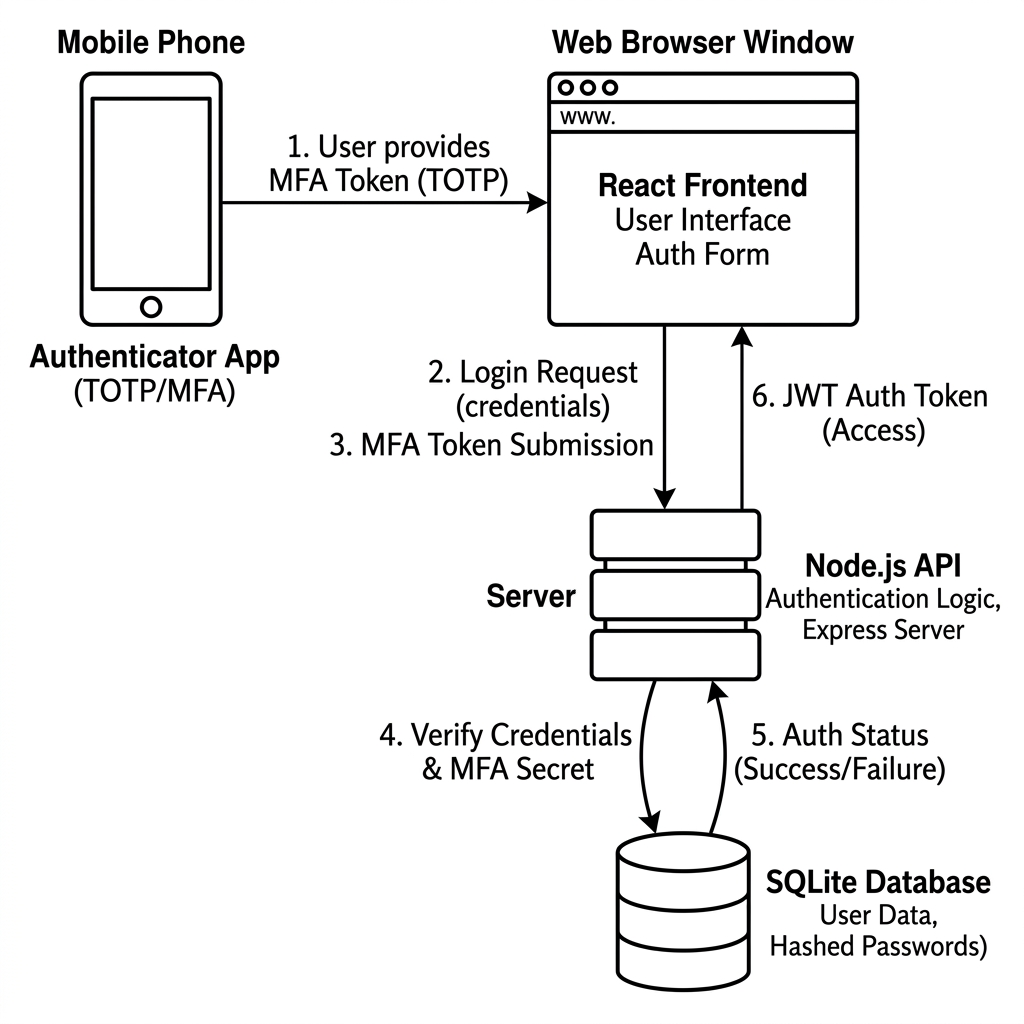
\includegraphics[width=0.8\textwidth]{images/mfa_architecture_diagram.png}
\caption{Diagrama de Arquitectura y Secuencia de Autenticación MFA}
\label{fig:arquitectura}
\end{figure}

\subsection{Flujo de Configuración Inicial (Setup 2FA)}
Para que la autenticación multifactor surta efecto, el usuario debe emparejar su cuenta con una aplicación de generación de tokens de un solo uso (TOTP). El proceso implementado sigue las pautas de seguridad recomendadas:
\begin{enumerate}
    \item \textbf{Generación Criptográfica:} Al solicitar el registro MFA, la API de Node.js emplea la librería \texttt{otplib} para generar una semilla criptográfica pseudoaleatoria única en Base32 (el \textit{Secret}).
    \item \textbf{Asociación URI y QR:} El backend construye un URI compatible con el formato estándar `otpauth://totp/...` que incluye el nombre del usuario, el \textit{Issuer} (``SecurityAgentApp'') y la semilla generada. Esta URI se convierte en una imagen de código QR en base64 usando la librería \texttt{qrcode}.
    \item \textbf{Transmisión Segura:} El secreto y el código QR se envían al frontend a través de un canal que se presupone seguro (HTTPS en producción). Paralelamente, el secreto se almacena en la tabla del usuario en SQLite, y el estado `twofaEnabled` se inicializa temporalmente en 0 (Pendiente de confirmación).
    \item \textbf{Confirmación Explícita:} El usuario escanea el código QR con su aplicación TOTP, que comienza a generar códigos rotativos de 6 dígitos cada 30 segundos. El usuario debe ingresar el código actual en la plataforma para probar la configuración.
    \item \textbf{Validación y Activación:} El servidor recibe el código, lo contrasta con el secreto almacenado ejecutando el algoritmo HMAC-SHA1 internamente. Si el código coincide (o se encuentra dentro de la ventana de tolerancia temporal por latencia de reloj), la bandera `twofaEnabled` se actualiza a 1 (Activo) en la base de datos de manera atómica.
\end{enumerate}

\subsection{Flujo de Autenticación con 2FA Activo}
Una vez el usuario ha activado su configuración, el proceso de inicio de sesión se divide lógicamente y temporalmente en dos fases:
\begin{itemize}
    \item \textbf{Fase 1 (Autenticación Primaria):} El usuario envía su correo electrónico y contraseña en texto plano (que viajan protegidos por TLS). El backend busca al usuario por su índice de correo en SQLite. Se utiliza el algoritmo adaptativo `bcrypt` para validar que el hash almacenado corresponde a la contraseña proveída. Si las credenciales son válidas y el usuario tiene 2FA activo, el servidor \textbf{no} expide un JWT definitivo. En su lugar, responde con un payload especial `{ status: '2FA_REQUIRED', userId: id }`. El usuario está parcialmente autenticado pero carece de autorización para acceder a recursos.
    \item \textbf{Fase 2 (Validación TOTP):} El frontend presenta un modal secundario solicitando el código dinámico al usuario. Este ingresa los 6 dígitos arrojados por su aplicación Authenticator. El frontend envía la solicitud POST al endpoint `/api/auth/2fa/login-verify` con el `userId` y el `code`. El backend recupera el `twofaSecret` de la base de datos asociado al `userId` y utiliza \texttt{otplib.authenticator.check(code, secret)} para la evaluación final. Únicamente bajo una validación exitosa, el servidor firma y entrega un Token JWT válido por 24 horas, permitiendo al usuario consumir el catálogo de productos y emitir órdenes de compra a través del componente \texttt{Dashboard.tsx}.
\end{itemize}


\section{Herramientas Tecnológicas Seleccionadas}

El desarrollo del prototipo implicó la cuidadosa selección de librerías y tecnologías de código abierto maduras, reconocidas ampliamente por la industria y que aseguran el cumplimiento de estándares criptográficos (como RFC 6238 y bcrypt). La siguiente tabla enumera y justifica las decisiones arquitectónicas principales:

\begin{table}[H]
    \centering
    \renewcommand{\arraystretch}{1.5}
    \begin{tabularx}{\textwidth}{@{} l >{\raggedright\arraybackslash}X >{\raggedright\arraybackslash}X @{}}
        \toprule
        \textbf{Componente / Rol} & \textbf{Tecnología Elegida} & \textbf{Justificación Técnica y de Seguridad} \\
        \midrule
        \textbf{Runtime de Backend} & Node.js con Express.js & Ofrece un ecosistema de librerías de seguridad asíncronas muy rico, procesamiento eficiente de E/S y fácil manejo de cabeceras CORS e interceptación de tokens mediante middlewares personalizados. \\
        \textbf{Motor de Base de Datos} & SQLite3 & Sistema relacional embebido libre de configuración, ideal para prototipos. Permite almacenar hashes binarios y textos asegurando consistencia atómica sin desplegar clusters pesados. \\
        \textbf{Framework de Frontend} & React 18 con TypeScript y Vite & Garantiza tipado estático riguroso y evita errores de tiempo de ejecución mediante comprobaciones de Typescript. React facilita la construcción de UI basadas en estados, fundamental para separar la vista de login, el modal 2FA y el dashboard transaccional de forma fluida. \\
        \textbf{Cifrado de Contraseñas} & \texttt{bcryptjs} & Algoritmo de hash adaptativo (key derivation function) con factor de trabajo (salt rounds) configurable (se estableció en 10). Diseñado para mitigar ataques de diccionario y de hardware especializado (GPU/ASIC) al ralentizar intencionalmente el tiempo de cómputo. \\
        \textbf{Manejo de Sesiones} & \texttt{jsonwebtoken} (JWT) & Tokens stateless (sin almacenamiento de sesión en servidor). El servidor firma digitalmente el token con una clave secreta HMAC-SHA256 (\texttt{JWT\_SECRET}), previniendo cualquier manipulación de la identidad o elevación de privilegios en el lado del cliente (tampering). \\
        \textbf{Motor MFA / TOTP} & \texttt{otplib} & Librería estandarizada y auditada en el ecosistema NPM para generar algoritmos de contraseña de un solo uso basados en HMAC (HOTP) y basados en tiempo (TOTP). Soporta mitigaciones como ventanas temporales ajustables (window drift). \\
        \textbf{Generador de QR} & \texttt{qrcode} & Facilita la adopción por parte del usuario final generando dinámicamente imágenes Base64 de códigos bidimensionales que pueden ser escaneados de manera segura dentro de la propia intranet sin recurrir a APIs externas inseguras (evitando filtraciones de secretos en URLs). \\
        \textbf{Diseño e Interfaz} & CSS Modular e Íconos \texttt{lucide-react} & Otorga un acabado estético moderno al portal simulado, utilizando variables globales para soportar paletas de colores legibles y animaciones que reducen la fricción operativa del usuario durante los pasos críticos de validación. \\
        \bottomrule
    \end{tabularx}
    \caption{Relación de Tecnologías e Implicaciones de Seguridad}
    \label{tab:herramientas}
\end{table}

\section{Detalles Técnicos de la Implementación}

A fin de ilustrar la rigurosidad técnica del desarrollo, se procede a analizar fragmentos y esquemas clave correspondientes al código fuente original del proyecto.

\subsection{Esquema de Persistencia y Modelado de Datos}

La seguridad inicia en el diseño del modelo de datos. En el archivo `backend/db.js`, la tabla `users` está deliberadamente estructurada para almacenar credenciales transformadas criptográficamente.

\begin{lstlisting}[language=SQL, caption={Definición de la estructura de usuarios y controles 2FA}]
CREATE TABLE IF NOT EXISTS users (
    id INTEGER PRIMARY KEY AUTOINCREMENT,
    name TEXT,
    address TEXT,
    phone TEXT,
    email TEXT UNIQUE,           -- Previene colisiones y enumeración masiva
    password TEXT,               -- Hash derivado usando bcrypt, NO texto plano
    twofaSecret TEXT,            -- Semilla Base32 asociada a la identidad
    twofaEnabled INTEGER DEFAULT 0 -- Bandera atómica de exigencia de segundo factor
);
\end{lstlisting}
Esta estructura garantiza que, incluso ante un evento de Inyección SQL que lograra exfiltrar el contenido de la base de datos, las contraseñas originales permanecen ininteligibles por la fortaleza del algoritmo `bcrypt` aplicado con factores de coste dinámicos.

\subsection{Middleware de Autorización y Manejo de JSON Web Tokens}

El diseño stateless requiere un verificador perimetral de identidad. Se implementó un \textit{Middleware} en Express.js (`server.js`, líneas 32-40) que intercepta el encabezado \texttt{Authorization: Bearer <token>} de toda petición a rutas protegidas (tales como visualización del catálogo o creación de órdenes).

\begin{lstlisting}[language=JavaScript, caption={Middleware de intercepción y verificación de sesión JWT}]
const authMiddleware = (req, res, next) => {
    const token = req.headers.authorization?.split(' ')[1];
    if (!token) return res.status(401).json({ error: 'No token provided' });
    
    // Verificación criptográfica de firma HMAC-SHA256
    jwt.verify(token, JWT_SECRET, (err, decoded) => {
        if (err) return res.status(401).json({ error: 'Invalid token' });
        req.user = decoded; // Inyección de la identidad confirmada para handlers subsiguientes
        next();
    });
};
\end{lstheaders}
\end{lstlisting}

\subsection{Generación del Factor Dinámico y Renderización del Código QR}

La configuración inicial es el punto más crítico del ciclo de vida del segundo factor, puesto que es el único momento en el que el secreto (semilla) y el servidor comparten el canal de comunicación. El endpoint `/api/auth/2fa/generate-qr` gestiona esta inicialización:

\begin{lstlisting}[language=JavaScript, caption={Algoritmo de inicialización MFA y emisión de códigos de vinculación}]
app.post('/api/auth/2fa/generate-qr', authMiddleware, async (req, res) => {
    try {
        const userId = req.user.id;
        const user = await getQuery('SELECT email FROM users WHERE id = ?', [userId]);
        
        // 1. Generación de semilla pseudoaleatoria base32
        const secret = otplib.authenticator.generateSecret();
        
        // 2. Construcción de URI según estándar para Google Authenticator
        const otpauth = otplib.authenticator.keyuri(
            user.email, 'SecurityAgentApp', secret
        );
        
        // 3. Persistencia temporal (pendiente de activación)
        await runQuery('UPDATE users SET twofaSecret = ?, twofaEnabled = 0 WHERE id = ?', 
                      [secret, userId]);
        
        // 4. Renderización del QR vectorizado libre de dependencias de terceros
        const qrCodeBase64 = await qrcode.toDataURL(otpauth);
        res.json({ qrCodeBase64, secret });
    } catch (err) {
        res.status(500).json({ error: err.message });
    }
});
\end{lstlisting}

\subsection{Implementación de la Regla de Negocio: Acceso Obligatorio con MFA}

En el lado del cliente, el componente \texttt{Dashboard.tsx} ilustra una política estricta de mitigación de daños (fail-secure). Al ingresar, el estado lógico de la aplicación condiciona la visualización. Si el parámetro `user.twofaEnabled` es falso, el portal prohíbe terminantemente la interacción con el catálogo o el carrito de compras.

\begin{lstlisting}[language=HTML, caption={Capa de vista en React y validación de bandera MFA}]
{!user?.twofaEnabled ? (
    <div className="alert alert-error">
        <ShieldAlert size={24} />
        <div>
            <strong>Acceso Denegado a la Tienda</strong>
            <p>Por motivos de seguridad, debes configurar la autenticación de dos pasos (2FA) antes de poder acceder al catálogo y realizar compras.</p>
        </div>
    </div>
    <ActivateMFA onComplete={() => setShowMFAConfig(false)} />
) : (
    <!-- Interfaz de la tienda Colombia Store -->
    <div className="glass-card">
        <h3>Bienvenido, {user?.name}</h3>
        <span className="badge-secure">Cuenta Segura</span>
    </div>
    <!-- Carga de productos... -->
)}
\end{lstlisting}

Este enfoque coercitivo en la capa de interfaz, respaldado intrínsecamente por la denegación de servicios en los endpoints de la API para usuarios sin la configuración finalizada, previene configuraciones débiles por omisión o desidia de los usuarios.

\section{Evaluación de Resultados y Análisis de Seguridad}

El despliegue de esta prueba de concepto proporciona datos concluyentes sobre cómo una arquitectura relativamente simple de integrar puede alterar drásticamente el modelo de amenazas de una aplicación web, logrando un balance favorable entre seguridad y usabilidad.

\subsection{Mejora Significativa en la Seguridad Preventiva}

La incorporación obligatoria de códigos TOTP altera fundamentalmente los requisitos que un cibercriminal debe reunir para comprometer cuentas dentro del portal:

\begin{enumerate}
    \item \textbf{Mitigación del Phishing a Escala:} En entornos de factor único (SFA), una campaña de correos fraudulentos que logre engañar a decenas de usuarios para que inserten su contraseña en un sitio apócrifo resulta en el control total e inmediato de sus cuentas. Con el sistema MFA implementado, el atacante requiere \textit{además} comprometer un código temporal de 6 dígitos. Dado que el código expira en una ventana nominal de 30 segundos, el atacante se enfrenta a una carrera de tiempo impracticable a gran escala, forzándolo a utilizar tácticas avanzadas y manuales de intermediación (Reverse Proxies y ataques MitM en tiempo real), las cuales son complejas de automatizar.
    \item \textbf{Inutilización de Bases de Datos Filtradas (Credential Stuffing):} Si un empleado u actor de amenazas externa comercializa una base de datos que contiene correos y contraseñas provenientes de brechas previas (Ej. LinkedIn, Adobe, Yahoo), los bots que intentan automáticamente probar dichos credenciales contra el endpoint `/api/auth/login` fracasarán sistemáticamente, ya que la API no entrega un JWT sin superar satisfactoriamente la validación `/api/auth/2fa/login-verify` que exige la posesión física del token generador.
    \item \textbf{Resistencia Criptográfica Interna:} La base de datos local SQLite se encuentra protegida contra violaciones de datos estáticos gracias al empleo del hash \texttt{bcryptjs} con múltiples iteraciones (salt rounds). Adicionalmente, se impide el secuestro de sesión mediante inyección de scripts cruzados (XSS) mediante la limitación de vigencia del JWT (establecida en 1 día o \texttt{1d}) en conjunción con validación de sintaxis de la librería y su almacenamiento en estructuras cerradas de memoria durante el ciclo de la SPA.
\end{enumerate}

\subsection{Evaluación de Fricción y Usabilidad}

Si bien un axioma conocido de la seguridad informática expone la existencia de una relación inversamente proporcional entre seguridad y conveniencia, el prototipo desarrollado mitiga el impacto negativo en la experiencia del usuario de las siguientes maneras:
\begin{itemize}
    \item \textbf{Interfaz Intuitiva y Cierre Estético:} Se empleó un diseño limpio utilizando íconos (\texttt{lucide-react}) y colores de semáforo cognitivo (tonos de urgencia en la exigencia de 2FA y tonos de verificación en verde para cuentas seguras). Las animaciones de transición limitan la carga cognitiva de los pasos de verificación.
    \item \textbf{Incorporación QR Estándar:} La compatibilidad total con aplicaciones de mercado ubicuas, gracias al uso formalizado del estándar `otpauth://`, permite a los usuarios configurar el mecanismo con aplicaciones que, muy probablemente, ya portan instaladas en sus teléfonos móviles.
    \item \textbf{Manejo Transparente de Fallos:} Los errores en la introducción de código derivan en notificaciones claras e inmediatas de validación vía la herramienta `sonner` de React, impidiendo estados de bloqueo fantasma u ocultos que desconcierten a los consumidores del portal.
\end{itemize}

\section{Evidencia de Funcionamiento del Prototipo}

A continuación se presentan capturas de pantalla que evidencian el funcionamiento real del portal web y la implementación estricta del flujo MFA.

\begin{figure}[H]
    \centering
    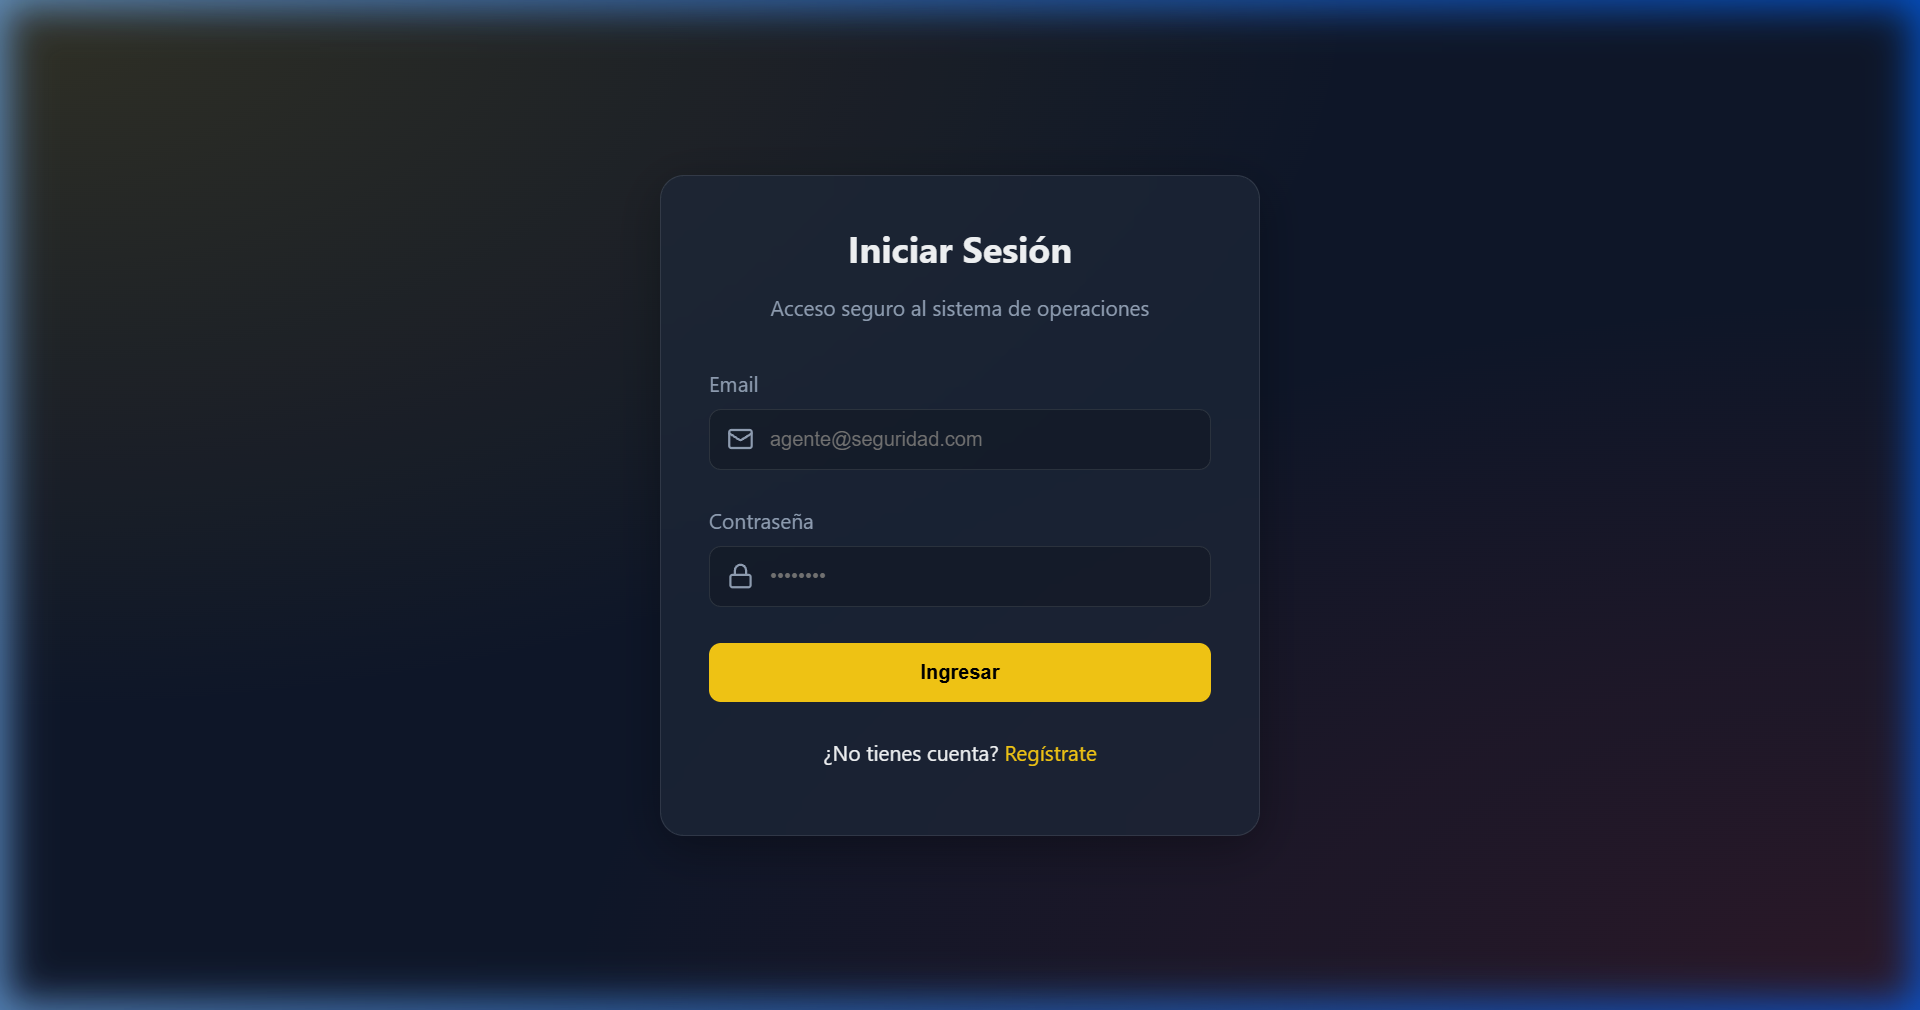
\includegraphics[width=0.8\textwidth]{images/login.png}
    \caption{Pantalla de inicio de sesión de Colombia Store.}
    \label{fig:login}
\end{figure}

\begin{figure}[H]
    \centering
    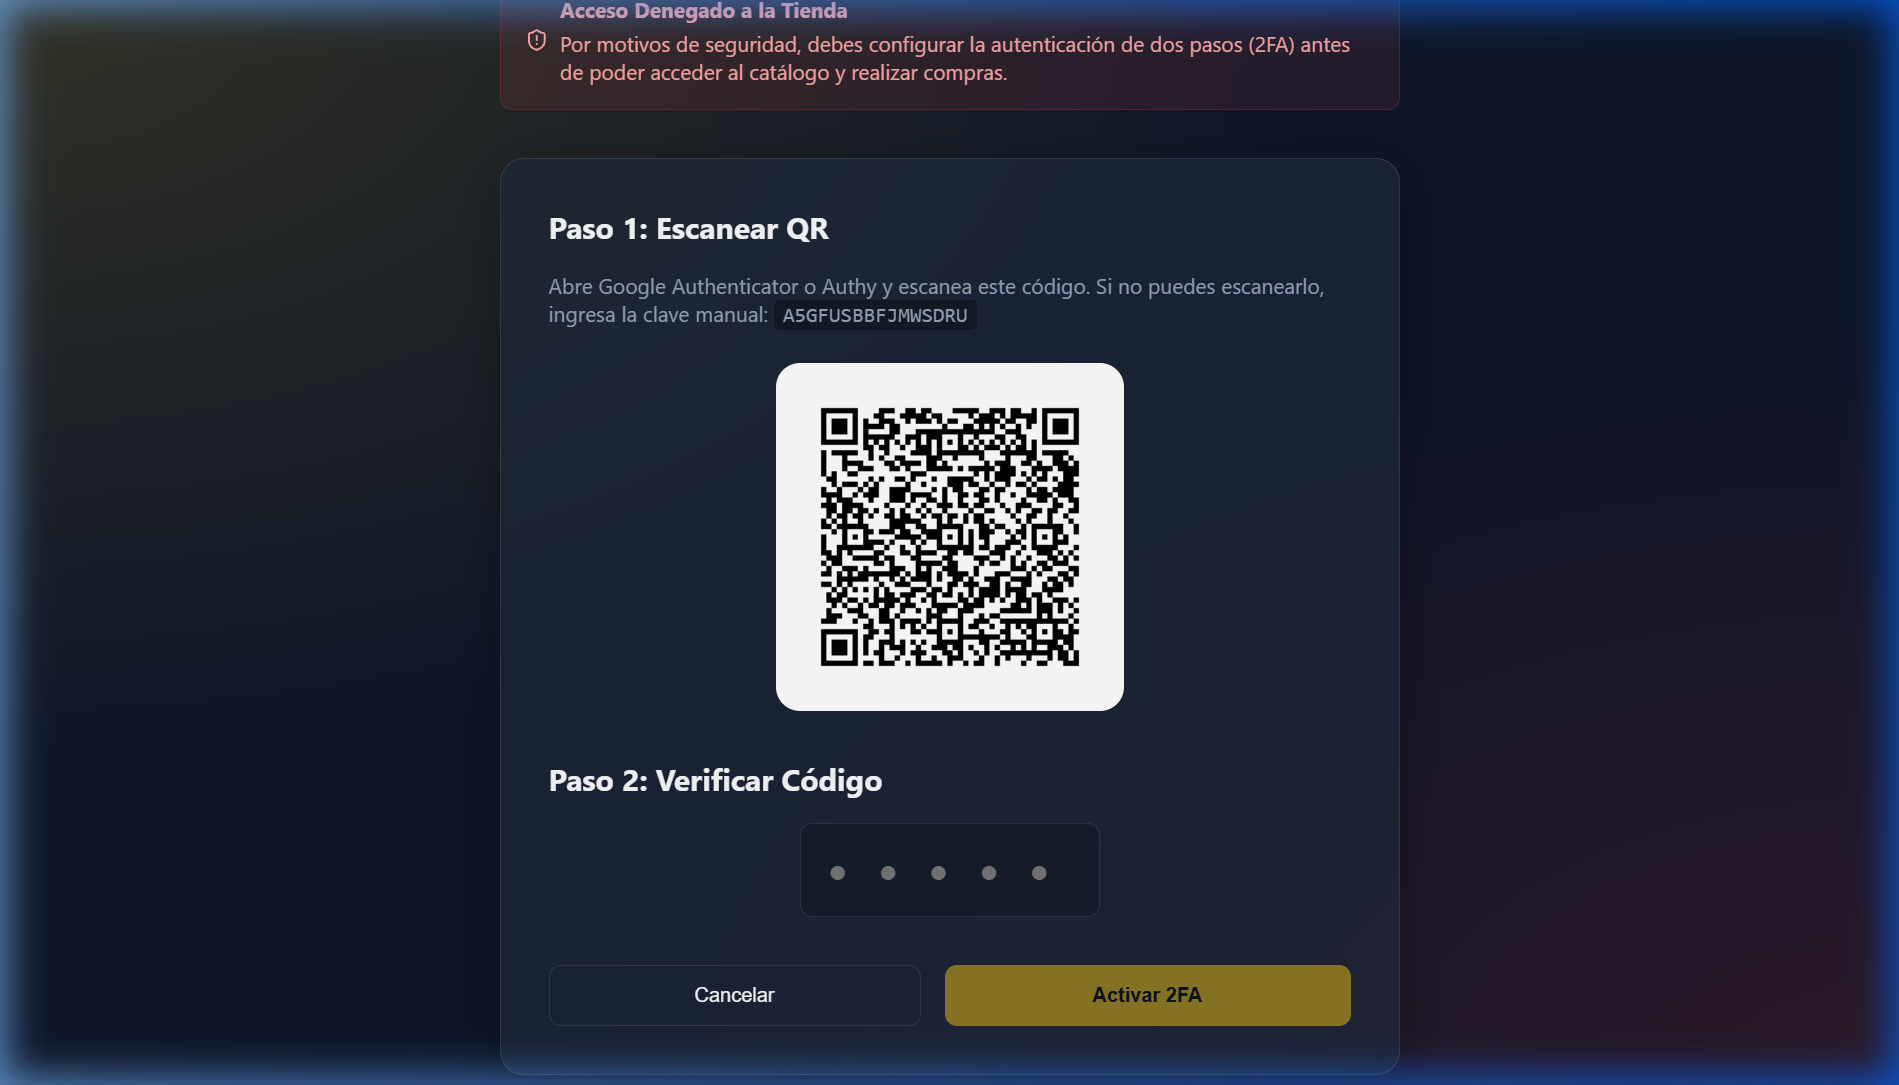
\includegraphics[width=0.8\textwidth]{images/qr.png}
    \caption{Bloqueo de acceso y presentación del código QR para vinculación TOTP.}
    \label{fig:qr}
\end{figure}

\begin{figure}[H]
    \centering
    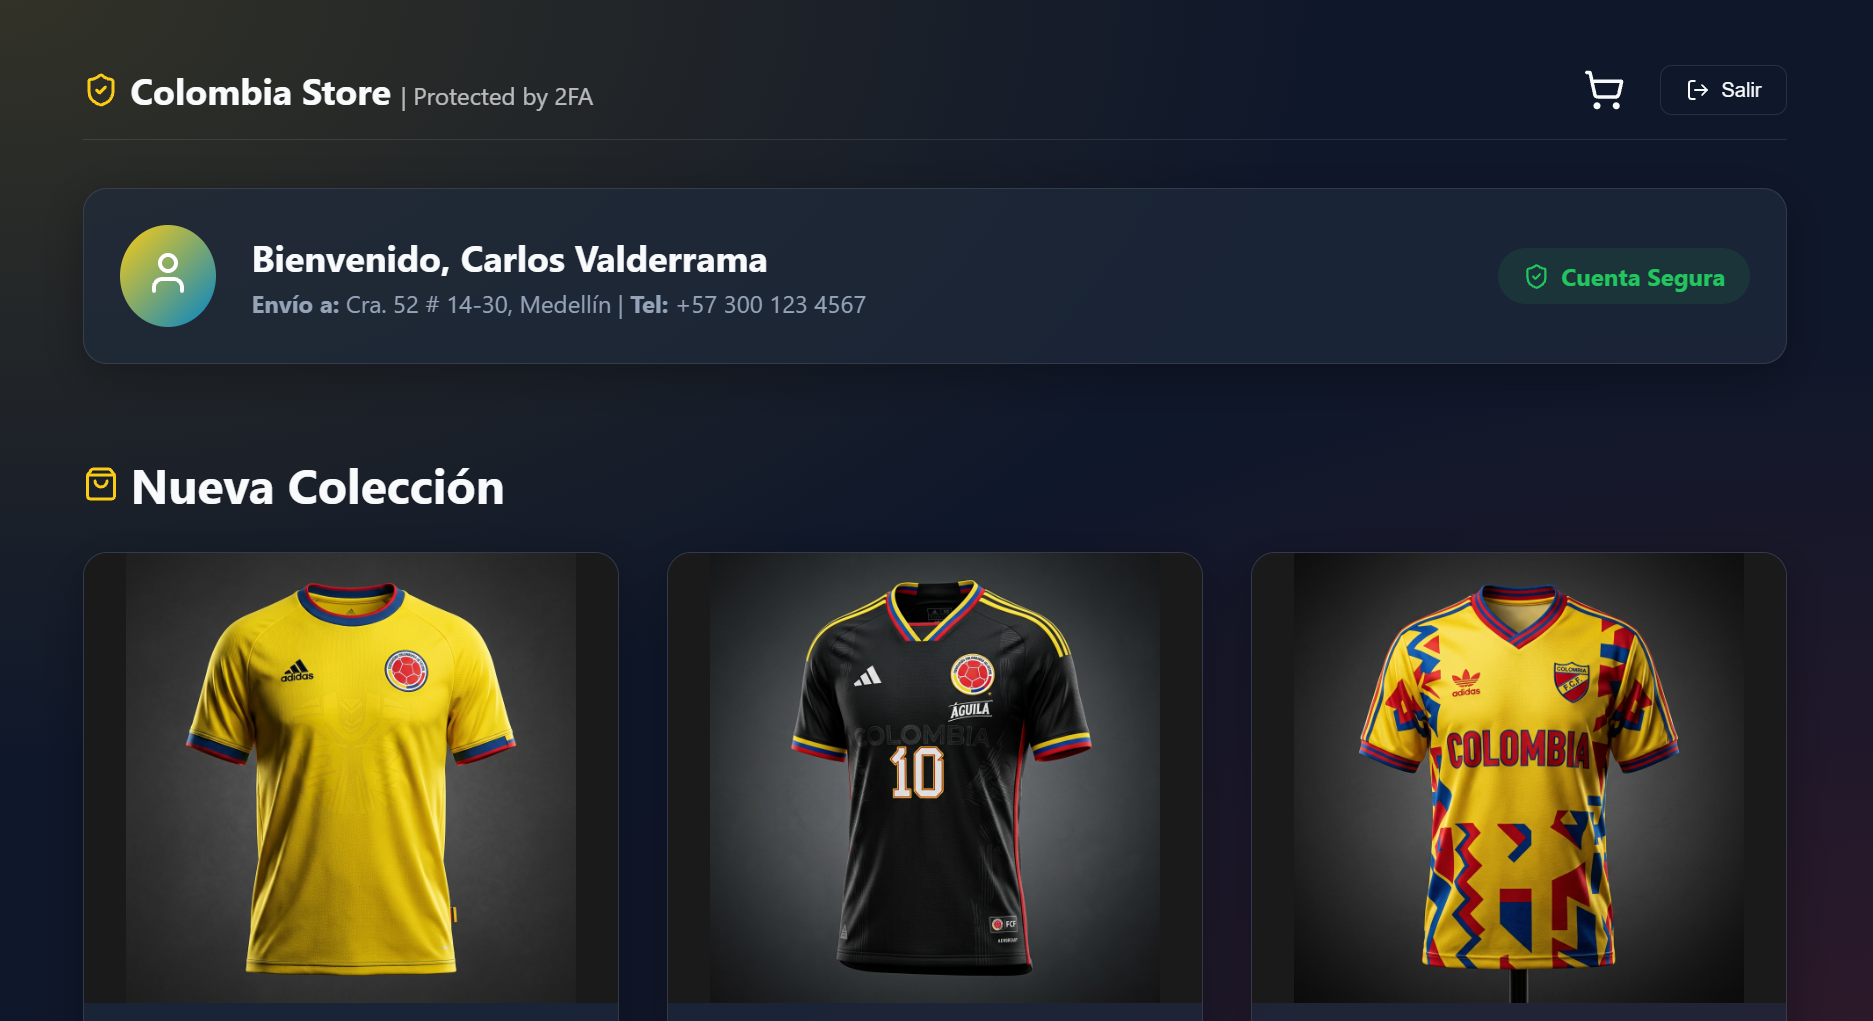
\includegraphics[width=0.8\textwidth]{images/dashboard.png}
    \caption{Acceso exitoso al catálogo tras verificación MFA.}
    \label{fig:dashboard}
\end{figure}

\begin{figure}[H]
    \centering
    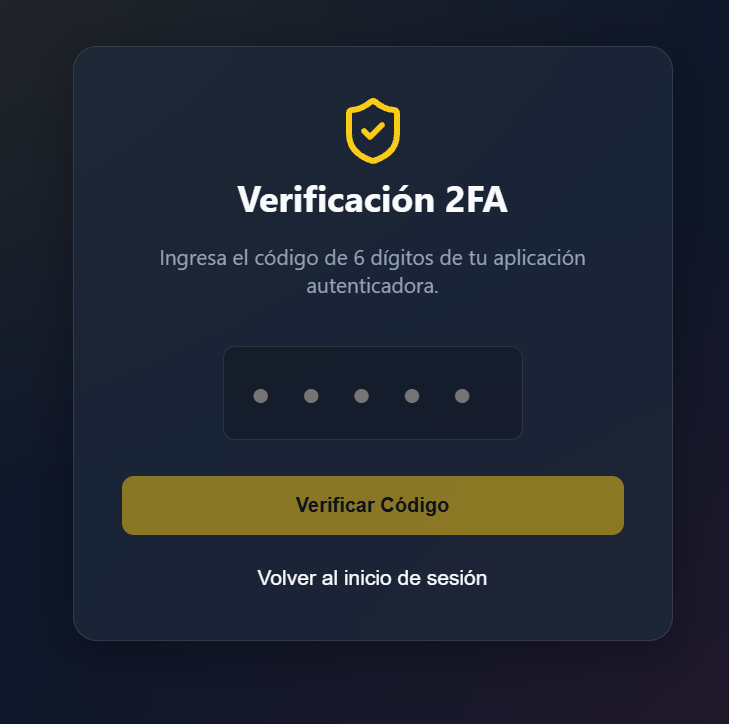
\includegraphics[width=0.8\textwidth]{images/login_2fa.png}
    \caption{Intercepción de inicio de sesión exigiendo el código TOTP temporal.}
    \label{fig:login_2fa}
\end{figure}

\section{Limitaciones y Posibles Mejoras Tecnológicas}

No obstante el innegable progreso obtenido en la postura de ciberseguridad, el prototipo y la arquitectura seleccionada ostentan ciertas limitaciones operativas que es pertinente identificar para abordar en iteraciones y pases a producción en infraestructuras de envergadura.

\subsection{Vulnerabilidades Remanentes}
\begin{itemize}
    \item \textbf{Ataques de Phishing en Tiempo Real (Adversary-in-the-Middle o AitM):} El esquema TOTP es susceptible a ataques sumamente sofisticados ejecutados mediante proxies inversos dinámicos como \textit{Evilginx2} o \textit{Modlishka}. Dichas herramientas suplantan el servidor real, interceptando simultáneamente la contraseña y el código de 6 dígitos del usuario durante su periodo breve de vida (30 segundos), permitiéndoles extraer y usurpar la cookie de sesión o JWT sin requerir vulnerar la criptografía matemáticamente.
    \item \textbf{Pérdida Crítica del Dispositivo (Single Point of Failure):} En la implementación actual, si un usuario extravía su teléfono móvil, o elimina accidentalmente la semilla del \textit{Authenticator}, queda imposibilitado indefinidamente para acceder a la aplicación. El sistema carece, de momento, de un mecanismo desatendido de restauración.
\end{itemize}

\subsection{Propuestas de Mejora Continua}
\begin{enumerate}
    \item \textbf{Implementación de Códigos de Respaldo (Backup / Recovery Codes):} Desarrollar una funcionalidad que genere criptográficamente de 8 a 10 cadenas alfanuméricas complejas de un solo uso en el momento de activación del 2FA. Se ordenaría al usuario imprimir o almacenar a buen resguardo estos códigos físicos, mitigando el bloqueo por pérdida de terminal.
    \item \textbf{Migración hacia Estándares Inmunizados contra Phishing (FIDO2 / WebAuthn):} La verdadera evolución del sistema implica la sustitución de códigos tipados estáticos de corta duración por el uso de tokens criptográficos asimétricos validados por hardware (Llaves FIDO, YubiKeys o Passkeys apoyadas en el TPM y biometría nativa del terminal como Windows Hello o Touch ID de Apple). Este estándar asegura al usuario frente a proxies MitM.
    \item \textbf{Defensas Antifraudulentas Activas:} Incluir un sistema de registro de eventos (Audit Logging), telemetría de fallos sucesivos y mecanismos de limitación de tasa (rate throttling o CAPTCHA invisible) frente a miles de intentos ciegos sobre el formulario de inserción del TOTP en el endpoint de validación.
\end{enumerate}

\section{Conclusiones Generales del Equipo}

El desarrollo y culminación de la prueba de concepto para la plataforma interactiva simulada ratifica palpablemente las directrices modernas de la seguridad orientada a identidad digital. Del proceso se obtienen las siguientes inferencias medulares:

\begin{enumerate}
    \item \textbf{Aplicabilidad Directa y Tangible:} La autenticación multifactor no es una tecnología reservada únicamente a grandes corporaciones con infraestructuras millonarias, sino un esquema accesible y fácilmente implementable utilizando librerías abiertas estándar (\texttt{otplib}, \texttt{jsonwebtoken}), cuyo coste de adopción para organizaciones medianas resulta mínimo en comparación al costo devastador que conllevan los ataques persistentes por robo de información y accesos corporativos.
    \item \textbf{Resiliencia Basada en Diversificación:} El principio de separar la posesión del secreto del conocimiento de este ha demostrado su total pertinencia. El ataque a una base de datos mal defendida deja de ser el vector de daño definitivo, al carecer el actor hostil del dispositivo físico del legítimo propietario. Se demuestra que una capa tecnológica interviniente (2FA Modal) frustra de raíz intentos oportunistas de usurpación masiva de accesos.
    \item \textbf{Diseño con Seguridad por Defecto:} A través del diseño implementado, se constata que imponer las restricciones directamente a nivel de las directivas de capa de red (Middleware) y de representación (React UI fail-safes) fomenta que la seguridad no sea una configuración de preferencia personal o algo "opcional", sino un eslabón incrustado en el ADN y reglas de negocio del software. Sin validación dual, el software deliberadamente no otorga servicio.
    \item \textbf{Reconocimiento de la Complejidad Criptográfica Asistida:} El trabajo subraya cómo las utilidades contemporáneas abstraen eficientemente las funciones avanzadas como HMAC, SHA1, codificación en Base32 e interpretación de QR. No obstante, recalca al estudiante y al desarrollador la necesidad crítica de preservar con extremada diligencia elementos como los tokens JWT y las claves \texttt{JWT\_SECRET} de variables de entorno, demostrando que la solidez matemática de la solución depende de que los desarrolladores protejan los cimientos estructurales.
\end{enumerate}

En síntesis, el prototipo cumple integralmente el propósito académico del proyecto final (Propuesta 2), materializando un escenario defensivo funcional que dota de confidencialidad e inmutabilidad estricta a un acceso web mediante la implementación concienzuda de autenticación de doble factor en el ámbito práctico y cotidiano de la tecnología transaccional web.

\vspace{1cm}
\begin{thebibliography}{9}
\bibitem{rfc6238} 
M'Raihi, D., Machani, S., Pei, M., \& Rydell, J. (2011). 
\textit{TOTP: Time-Based One-Time Password Algorithm} (RFC 6238). 
Internet Engineering Task Force (IETF).

\bibitem{owasp2021}
OWASP Foundation. (2021). 
\textit{OWASP Top 10: 2021 Identification and Authentication Failures}. 
Open Worldwide Application Security Project.

\bibitem{nist800}
Grassi, P. A., Garcia, M. E., \& Fenton, J. L. (2017). 
\textit{Digital Identity Guidelines} (NIST Special Publication 800-63B). 
National Institute of Standards and Technology.

\end{thebibliography}

\end{document}
